\documentclass[12pt]{article}\usepackage[]{graphicx}\usepackage[]{color}
%% maxwidth is the original width if it is less than linewidth
%% otherwise use linewidth (to make sure the graphics do not exceed the margin)
\makeatletter
\def\maxwidth{ %
  \ifdim\Gin@nat@width>\linewidth
    \linewidth
  \else
    \Gin@nat@width
  \fi
}
\makeatother

\definecolor{fgcolor}{rgb}{0.345, 0.345, 0.345}
\newcommand{\hlnum}[1]{\textcolor[rgb]{0.686,0.059,0.569}{#1}}%
\newcommand{\hlstr}[1]{\textcolor[rgb]{0.192,0.494,0.8}{#1}}%
\newcommand{\hlcom}[1]{\textcolor[rgb]{0.678,0.584,0.686}{\textit{#1}}}%
\newcommand{\hlopt}[1]{\textcolor[rgb]{0,0,0}{#1}}%
\newcommand{\hlstd}[1]{\textcolor[rgb]{0.345,0.345,0.345}{#1}}%
\newcommand{\hlkwa}[1]{\textcolor[rgb]{0.161,0.373,0.58}{\textbf{#1}}}%
\newcommand{\hlkwb}[1]{\textcolor[rgb]{0.69,0.353,0.396}{#1}}%
\newcommand{\hlkwc}[1]{\textcolor[rgb]{0.333,0.667,0.333}{#1}}%
\newcommand{\hlkwd}[1]{\textcolor[rgb]{0.737,0.353,0.396}{\textbf{#1}}}%
\let\hlipl\hlkwb

\usepackage{framed}
\makeatletter
\newenvironment{kframe}{%
 \def\at@end@of@kframe{}%
 \ifinner\ifhmode%
  \def\at@end@of@kframe{\end{minipage}}%
  \begin{minipage}{\columnwidth}%
 \fi\fi%
 \def\FrameCommand##1{\hskip\@totalleftmargin \hskip-\fboxsep
 \colorbox{shadecolor}{##1}\hskip-\fboxsep
     % There is no \\@totalrightmargin, so:
     \hskip-\linewidth \hskip-\@totalleftmargin \hskip\columnwidth}%
 \MakeFramed {\advance\hsize-\width
   \@totalleftmargin\z@ \linewidth\hsize
   \@setminipage}}%
 {\par\unskip\endMakeFramed%
 \at@end@of@kframe}
\makeatother

\definecolor{shadecolor}{rgb}{.97, .97, .97}
\definecolor{messagecolor}{rgb}{0, 0, 0}
\definecolor{warningcolor}{rgb}{1, 0, 1}
\definecolor{errorcolor}{rgb}{1, 0, 0}
\newenvironment{knitrout}{}{} % an empty environment to be redefined in TeX

\usepackage{alltt}

% make wider margins
\usepackage[margin=1in]{geometry}


%%%%%%%%%%%%%%%%%%%%%%%%%%%%%%%%%%%%%%%%%%%%%%%%%%%%%%%%%%%%%%%%
%
% Formatting
%
%%%%%%%%%%%%%%%%%%%%%%%%%%%%%%%%%%%%%%%%%%%%%%%%%%%%%%%%%%%%%%%%
  
% define font
\usepackage{times}

% math symbols
\usepackage{amsmath, amsfonts, amssymb, bbm, bm}

% extra graphics and figures formatting and options
\usepackage{graphicx,caption,subcaption,rotating,float,rotating,calc,fancyhdr,url,tablefootnote, titlesec,titletoc,arydshln}

% bullet lists, etc. with custom indentation
\usepackage{enumerate}

% easy in-text citations and colored urls
% \usepackage[colorlinks = true,
%             linkcolor = blue,
%             urlcolor  = blue,
%             citecolor = blue,
%             anchorcolor = blue]{hyperref}

% tell latex to not hyphenate words!!!
%\usepackage[none]{hyphenat}

% let equations spill over multiple pages
\allowdisplaybreaks

%line and sentence spacing and page formatting
% \usepackage[tablesfirst,notablist]{endfloat}
\usepackage{setspace,lineno,breakcites,booktabs}
\usepackage[title]{appendix}
\doublespace

%tikz package for drawing on matrixes
\usepackage{tikz}
\usetikzlibrary{matrix,arrows,positioning,cd}

%captions formatting
%\usepackage[small,it]{caption}
%\addtolength{\belowcaptionskip}{-3mm}
%\addtolength{\abovecaptionskip}{-3mm}
%\addtolength{\intextsep}{-3mm}

%bibliography
\usepackage[authoryear]{natbib}
\bibliographystyle{ecology}

%Miscellaneous formatting for paper
\newcommand*\mystrut[1]{\vrule width0pt height0pt depth#1\relax}
\providecommand{\keywords}[1]{\textbf{Key Words:} #1}
\renewcommand{\refname}{Literature Cited} 

%Define math operators myself
\newcommand\Tau{\mathcal{T}}
\DeclareMathOperator{\dbin}{binomial}
\DeclareMathOperator{\dpois}{Poisson}
\DeclareMathOperator{\dnorm}{normal}
\DeclareMathOperator{\dlnorm}{lognormal}
\DeclareMathOperator{\dgamma}{gamma}
\DeclareMathOperator{\dunif}{uniform}
\DeclareMathOperator{\dmultinom}{multinomial}
\DeclareMathOperator{\dbeta}{beta}
\DeclareMathOperator{\ddirch}{Dirichlet}
\DeclareMathOperator{\dbern}{Bernoulli}


%supressing warnings about bad boxes
\hfuzz=2pt
\vfuzz=2pt


%Adding multiple authors with multiple affiliations
\usepackage{authblk}

%Making key words heading
\providecommand{\keywords}[1]{\textbf{Key Words:} #1}


%%%%%%%%%%%%%%%%%%%%%%%%%%%%%%%%%%%%%%%%%%%%%%%%%%%%%%%%%%%%
%%%
%%% Title, Authorship
%%%
%%%%%%%%%%%%%%%%%%%%%%%%%%%%%%%%%%%%%%%%%%%%%%%%%%%%%%%%%%%%

\title{Draft - Integrated Population Model Development for White-tailed Deer in WI}

\author[1]{Alison C. Ketz \thanks{Email address: \texttt{aketz@wisc.edu}}}
\affil{Department of Forest and Wildlife Ecology, University of WI, Madison USA 53706}

 
\setcounter{Maxaffil}{0}

%%%%%%%%%%%%%%%%%%%%%%%%%%%%%%%%%%%%%%%%%%%%%%%%%%%%%%%%%%%%
%%%
%%% Begin Document
%%%
%%%%%%%%%%%%%%%%%%%%%%%%%%%%%%%%%%%%%%%%%%%%%%%%%%%%%%%%%%%%
\IfFileExists{upquote.sty}{\usepackage{upquote}}{}
\begin{document}
% print document title
\maketitle


%%%%%%%%%%%%%%%%%%%%%%%%%%%%%%%%%%%%%%%%%%%%%%%%%%%%%%%%%%%%
%%%
%%% Load libraries and set up cache
%%%
%%%%%%%%%%%%%%%%%%%%%%%%%%%%%%%%%%%%%%%%%%%%%%%%%%%%%%%%%%%%



%%%%%%%%%%%%%%%%%%%%%%%%%%%%%%%%%%%%%%%%%%%%%%%%%%%%%%%%%%%%
%%%
%%% Load parameter estimate data objects
%%%
%%%%%%%%%%%%%%%%%%%%%%%%%%%%%%%%%%%%%%%%%%%%%%%%%%%%%%%%%%%%

% load all simulation results objects for all years



%%%%%%%%%%%%%%%%%%%%%%%%%%%%%%%%%%%%%%%%%%%%%%%%%%%%%%%%%%%%
%%%
%%% Introduction
%%%
%%%%%%%%%%%%%%%%%%%%%%%%%%%%%%%%%%%%%%%%%%%%%%%%%%%%%%%%%%%%

\section{Introduction}

There are numerous research questions driving the present study of white-tailed deer in the core area of southcentral Wisconsin. Off the top of my head, I brainstormed some of these questions. We can cultivate a more targeted list for the paper going forward. 

Is chronic wasting disease (CWD) affecting the survival rate to a level that is reducing the population growth rate to unsustainable levels? Is CWD reducing recruitment and therefore reducing the population growth rate? Should there be changes in harvest to account for this additional source of mortality? Are there density dependent feedbacks with respect to recruitment that offset the mortality attributable to the disaese? CWD disproportionately affects males, which brings up the question as to what happens when there are greatly reduced numbers of males? Has there been a change in the stable stage distribution? What are the long term consequences of these changes, if any. What is the relationship between predation and mortality from CWD? Does predation reduce prevalence as simulations have shown?

CWD was first detected in 2001 from a hunter harvested deer. Shortly thereafter prevalence was estimated at 3\% in close vicinity to the focal case. Since then, CWD has spread from the initial focus and prevalence has increased to approximately 20\% in adult females and 40\% in adult males in the core area. Previous models indicated that population level effects would emerge when prevalence became sufficiently high. Etc...Etc.... 

There is obviously substantial more background to write in this section, although I am moving onto the technical detail of model development for the purpose of discussion and will fill in this background section when we get further along, likely after I write the review paper. Additional details to add to this introduction include:
\begin{itemize}
\item IPMs in general
\item Force of infection with spatial-temporal disease dynamics
\item CWD background
\item CWD population modeling work
\item novelty of our approach/bring it all together
\end{itemize}
 
%%%%%%%%%%%%%%%%%%%%%%%%%%%%%%%%%%%%%%%%%%%%%%%%%%%%%%%%%%%%
%%%
%%% Methods
%%%
%%%%%%%%%%%%%%%%%%%%%%%%%%%%%%%%%%%%%%%%%%%%%%%%%%%%%%%%%%%%

\section{Methods}

\subsection{Model description}

IPMs are generally constructed with three data sources, (1) population abundance, (2) survival from mark-recapture, and  (3) fecundity data, such as young of the year counts. In this present study, we have additional data sources related to the state transition of the disease process. I think we should at least initially approach this in a compartment model scenario with two classes: Susceptibles and Infected/Infectious.
\begin{enumerate}
\item Population counts or some other index of population size, 
\item Survival estimates from known fate collars 
\item Productivity metrics, such as pregnancy rates and fawn:doe ratios
\item Disease transmission from surveillence data
\end{enumerate}

Some advice from Kery and Schaub during the IPM workshop was to use a divide and conquer approach to get each aspect of the model working seperately before putting them altogether in the IPM. For now, we have our known fate model for survival already implemented to some extent. We still have to account for the transition of collared individuals to a positive disease status, even when they test negative at capture. 

In this draft, I have focused the most the population reconstruction, i.e. developing the age-at-harvest model. To begin, I have created a basic Directed Acyclyc Graph (DAG) as a jumping off point. This further aids in breaking down this large model into manageable size components (Figure \ref{fig:dag}).\\ 
\begin{sidewaysfigure}
\begin{center}
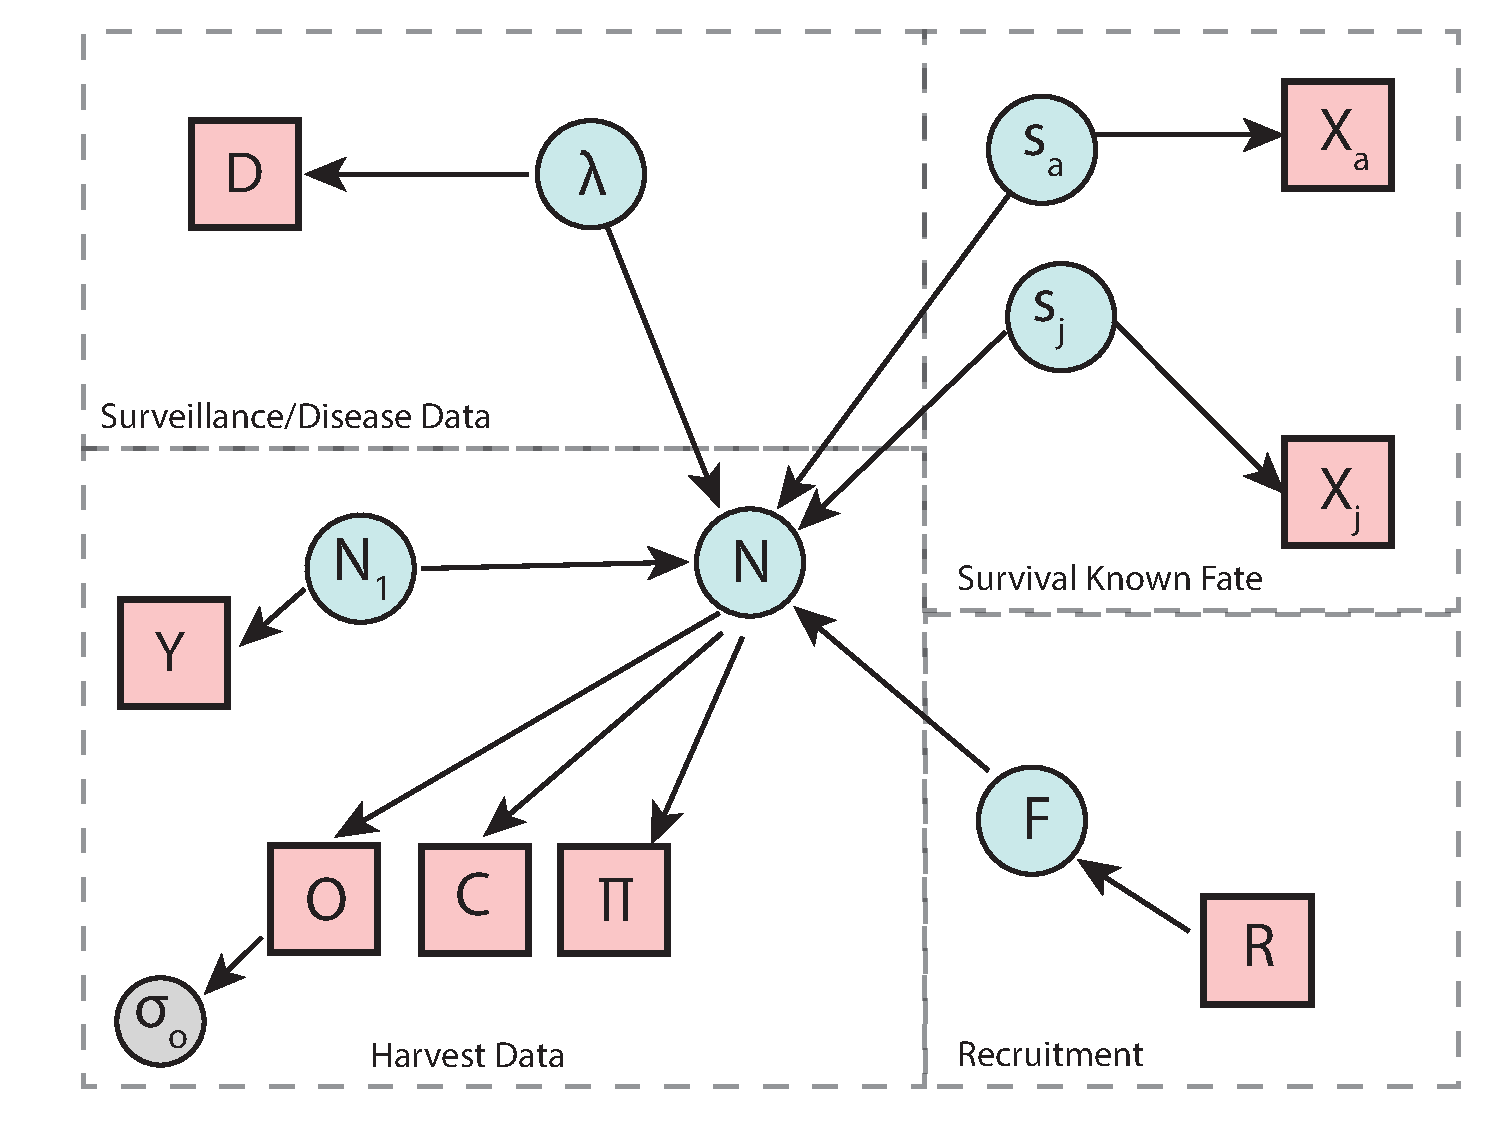
\includegraphics[width=10 in]{IPM_dag}
\caption{Directed Acyclic Graph of the Integrated Population Model incorporating state process parameters and data sources. Circles represent parameters, and squares represent data sources. Note that this is a simple preliminary graphic.}\label{fig:dag}
\end{center}
\end{sidewaysfigure}
\newpage
\subsection{Age-at-harvest population model}
Cross-sectional harvest data are used to reconstruct population abundances of cohorts through time, based on the latent process parameters described here.

\subsubsection{Process model}
We will assume a Markovian state process, where the total population size at time $t+1$ depends on the population at time $t$, and a function ($g$) of parameters governing the ecological processes of survival ($s$) and reproduction ($r$). Many population models also account for immigration and emigration, although for now, we make the simplifying assumption that the population is closed to these in/out processes. In general,
\begin{equation}
N_{t+1} = N_t \times g(s_t,r_t),
\end{equation} 
\noindent for year $t = 1,...,T$, where survival and recruitment can vary by year (or not). I think we should start the time step of the IPM in 2002. From 2002-2005, Mathews collected mark-recapture telemetry observations. We could use these data directly, or use the published rates as a prior for these years, which would be faster computationally. For the years we have collars deployed, 2017-2020, we can use the posterior predictive distributions to obtain survival for pre-hunt, hunting season, and post-hunt seasons. 

From 2005-2017, we'll have a 12 year period where we don't have mark-recapture data. We could average across the book-ending observations to obtain mean survival rates, assuming a constant survival for those in-between years. Similarly, provided the assumption of constant survival, we could use a moment-matched prior from the literature. 

Because we have data book-ending the timespan of the model, the first approach makes more sense. However, this makes the choice between re-analysis of the early data or using the already analyzed estimates as a prior. We can start with the latter, but if the credible intervals are too big for the derived annual survival, then we can make adjustments. We are working in a Bayesian framework, and using the prior-formulated approach will probably not alter the results all that much.

An annual timeline of events, similar to \citet{fieberg2010}, Figure 1(A), was created to help with formulating important phenomenon pertaining to the annual life cycle considering surveys/collaring, harvest, and the birth pulse (Figure \ref{fig:timeline}). We begin the increment of the model at the birth pulse, specifying intialization of the model on May 15. Thus, individuals transition into the next age class on this date every year the model is run. We can obtain survival based on the time to event analysis using the julian date of May 15 through approximately September 15, for when hunter harvest starts. This techinically varies each year, but only by a day or 2. This is actually a revision from the previous draft I sent, and aligns better with the age-at-harvest literature, and is easier to justify/conceptualize.

\begin{figure}[H]
\begin{center}
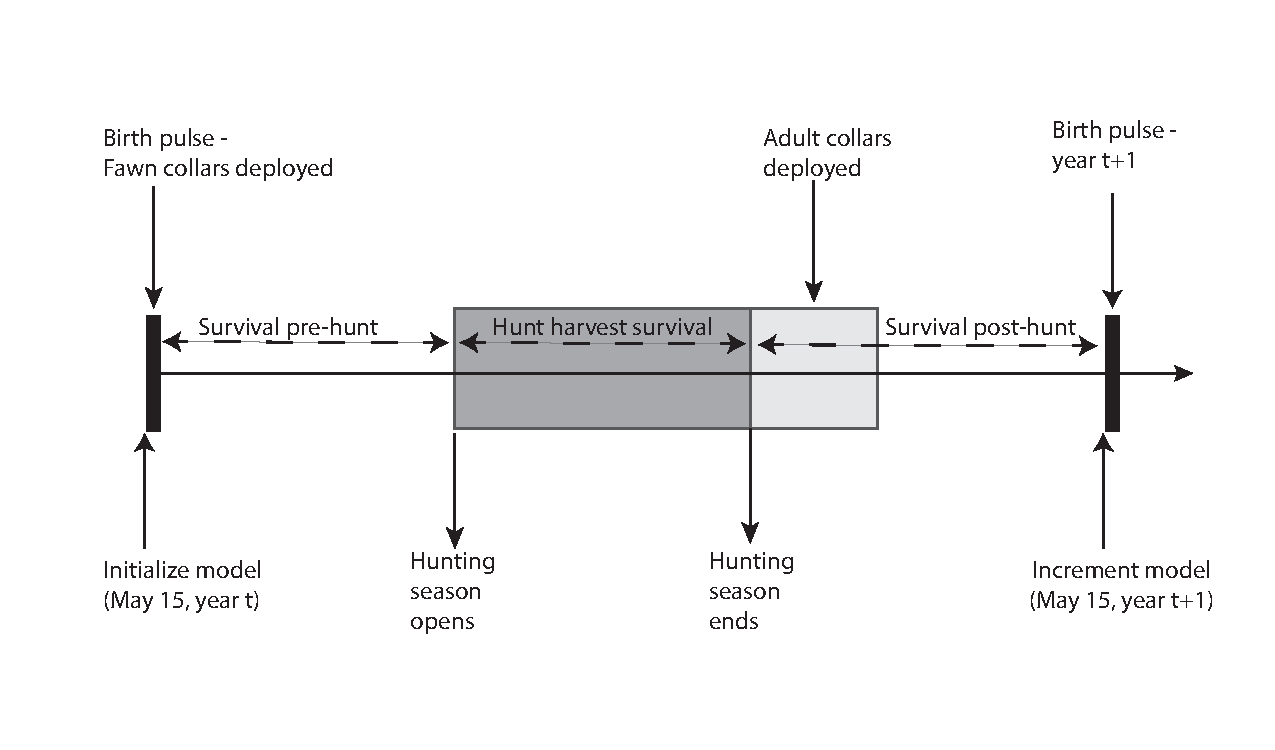
\includegraphics[width=6 in]{IPM_timeline}
\caption{Schematic of the age-at-harvest IPM annual timeline of events. Note that we may need to include population predictions prior to harvest and after population prediciton after harvest.}\label{fig:timeline}
\end{center}
\end{figure}

We condition on an intial population size in year 1, to reconstruct the population sizes from harvested individuals thereafter. The simplified population reconstruction using age-at-harvest data from \citet{fieberg2010} and \citet{gast2013b} is given by
% \begin{equation}
\begin{figure}[H]
\center
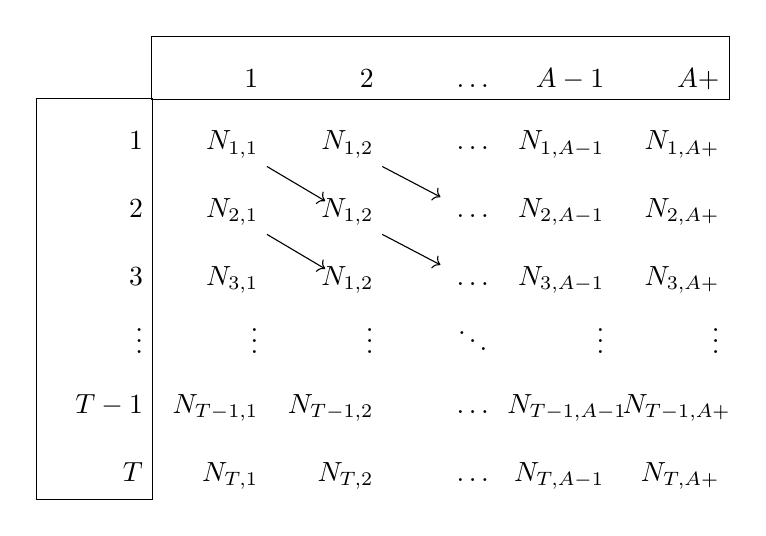
\begin{tikzpicture}
 \matrix (m)[
    matrix of math nodes,
    nodes in empty cells,
nodes={text width=3.5em,text height=1.5em, align=right}
]{
 & 1 & 2 & \dots & A-1 & A+\\
1 &  N_{1,1} & N_{1,2} & \dots & N_{1,A-1} & N_{1,A+} \\
2 &  N_{2,1} & N_{1,2} & \dots & N_{2,A-1} & N_{2,A+} \\
3 & N_{3,1} & N_{1,2} & \dots & N_{3,A-1} & N_{3,A+} \\
\vdots &  \vdots & \vdots & \ddots & \vdots & \vdots \\
T-1 &  N_{T-1,1} & N_{T-1,2} & \dots & N_{T-1,A-1} & N_{T-1,A+} \\
T &  N_{T,1} & N_{T,2} & \dots & N_{T,A-1} & N_{T,A+} \\
 };
 \draw (m-2-6.north-|m-1-1.west) rectangle (m-2-1.east|-m-7-2.south);
 \draw (m-1-2.north-|m-1-2.west) rectangle (m-1-6.east|-m-1-6.south);
\draw[->] (m-3-3.north-|m-3-3.west) -- (m-3-3.south |-m-3-3.east);
\draw[->] (m-4-3.north-|m-4-3.west) -- (m-4-3.south |-m-4-3.east);
\draw[->] (m-3-3.north-|m-4-4.west) -- (m-3-4.south |-m-3-4.east);
\draw[->] (m-4-4.north-|m-4-4.west) -- (m-4-4.south |-m-4-4.east);


\end{tikzpicture}
\end{figure}
% \end{equation}
Please note that there are various boxes and arrows that need to be added to this matrix, but I didn't want to spend the time this week to figure out tikz, although I will complete that going forward.

The following simplified life history diagram only incorporates disease status, age, and sex. I've omitted study area because this model grows in dimension quickly, so it was difficult work through all dimensions corresponding to the life history flow graphic. I couldn't think of a better way to demonstrate all of the state processes without getting even messier. Ultimately this model is founded in a leslie matrix formulation, so all of the assumptions of that modeling framework apply here, for example, Malthusian population growth, etc. 

\begin{figure}[H]
\begin{center}
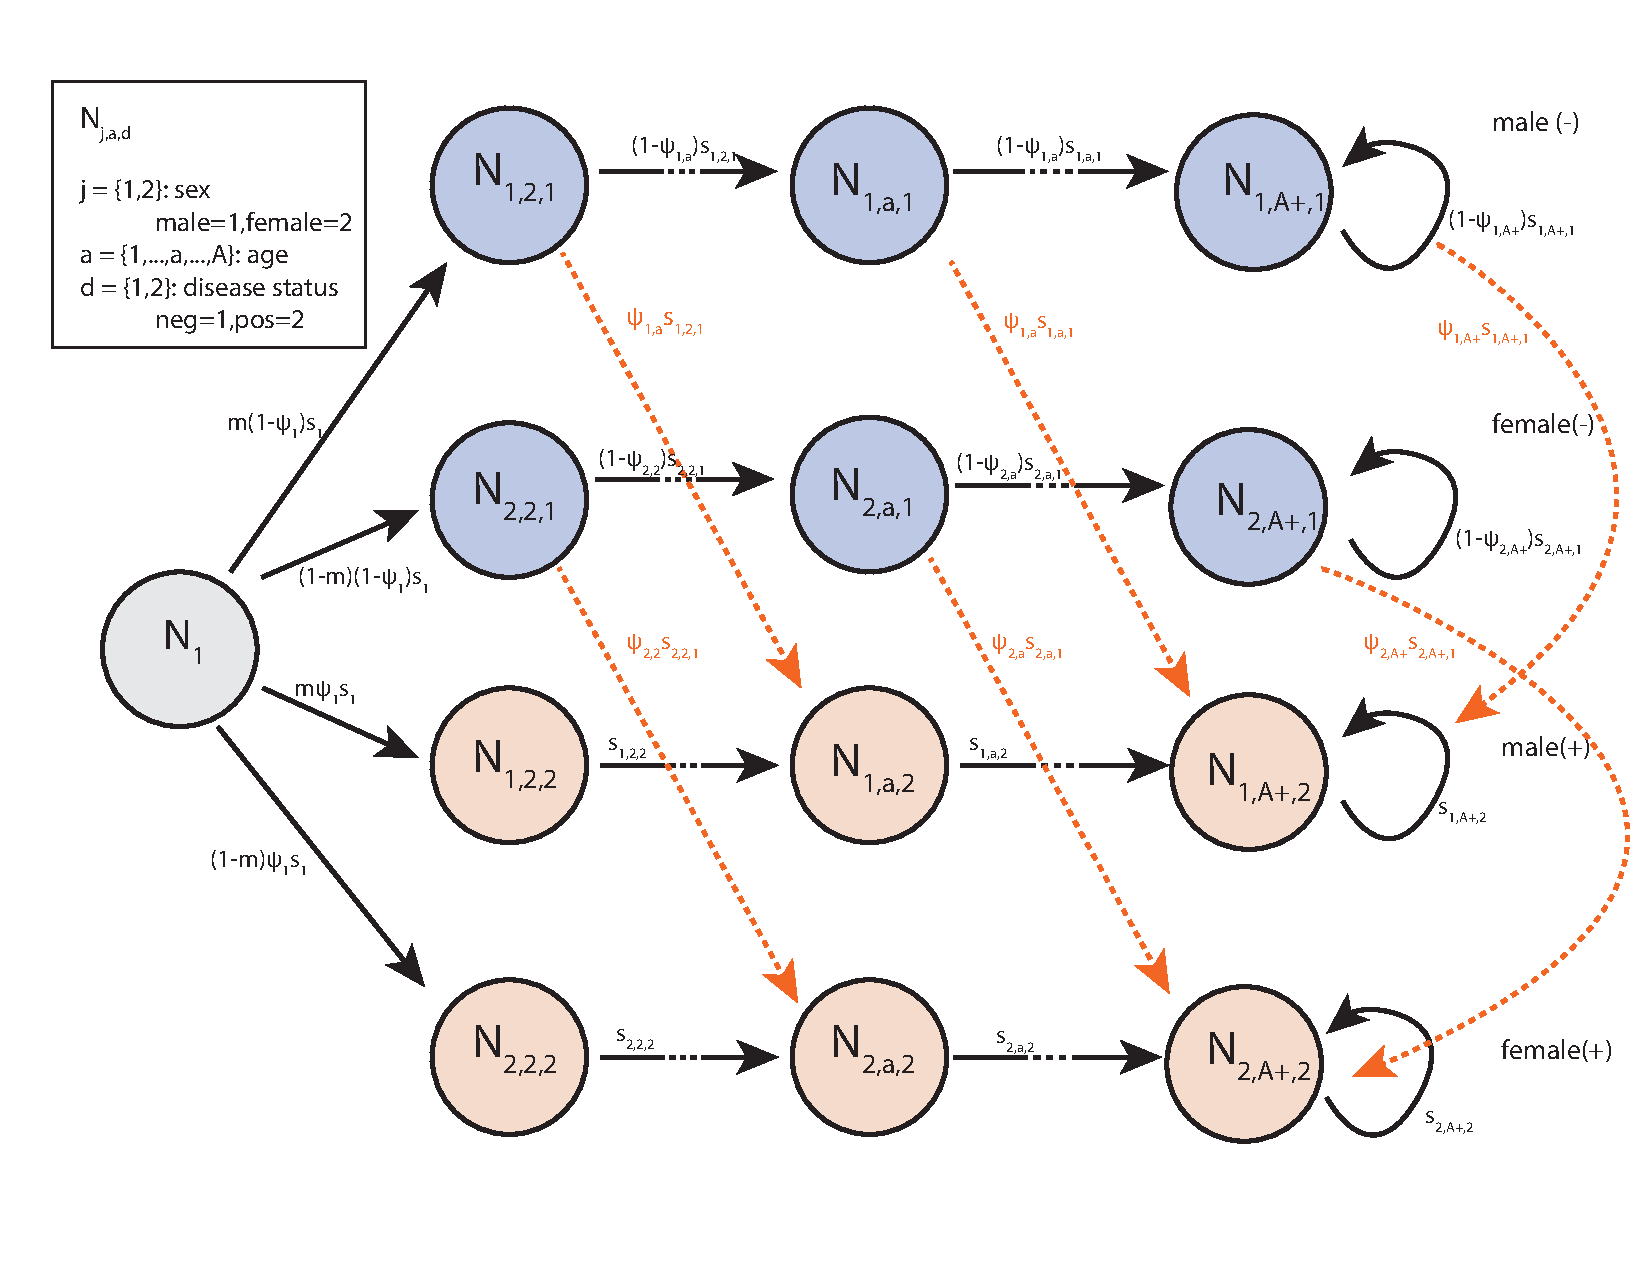
\includegraphics[width=6.5 in]{IPM_lifecycle}
\caption{Lifecycle diagram for an individual white-tailed deer as they progress through ages $a$, for sex $j$ and disease status $d$, where $m=.5$ is the proportion of sexless juveniles that are males.}\label{fig:Lifecylce}
\end{center}
\end{figure}

We will separate mortality during the hunting season, including bow and gun, from natural mortality outside of hunter harvest. Predicted ``true" abundance for each state variable is given by a series of two equations. The second equation is necessary to account for the terminal age class, denoted ($A+$) representing the fact that individuals that are 12.5 years of age or older remain in that age class.
\begin{align}
N_{t+1,j,a+1,d,k} & = N_{t,j,a,d,k}*S_{t,j,a,d}*(1-h_{t,j,k}) \text{ for } 1 \geq a < A-1,\\
N_{t+1,j,A+,d,k} & = N_{t,j,A-1,d,k}*S_{t,j,A-1,d}*(1-h_{t,j,A-1,k}) + N_{t,j,A+,d,k}*S_{t,j,A+,d}*(1-h_{t,j,A+,k}). 
\end{align}

\begin{table}[H]
\caption{The parameters in the population process model can vary across numerous states, resulting in a high dimensional matrix model.}
\begin{tabular}{l c l}
  Dimension & Index Notation & Range \\
  \hline
  Year & $t$ & $\{1,\dots,T=17\},\text{ corresponding to }\{2002,\dots,2018\}$ \\
  Sex & $j$ & $\{1 = \text{Male},2=\text{Female}\}$\\
  Age & $a$ & $\{1 = .5 \text{ year at harvest},\dots, A+=12.5 \text{ years or older}\}$\\
  Disease & $d$ &$\{1=\text{Negative},2=\text{Postive}\}$\\
  Study Area & $k$ & $\{1=\text{East},2=\text{West}\}$\\
  \hline
\end{tabular}
\end{table}

\noindent The true states of population abundance vary by year, sex, age, disease status, and study area. Natural mortality survival probabilities vary by sex, age, disease status, and year for the years with known-fate collar data. For the years prior to our framework, we could use the previous telemetry data. For years without any telemetry/GPS data we can make an aditional survival parameter that is constant for those years ``missing" auxiliary data. However, in all cases, we assume natural surival is constant across both study areas. This is flexible. The harvest probability varies by year, sex, age, and study area, and is assumed to be the same regardless of disease status \citep{grear2006}.

\subsubsection{Population data sources/description}
A challenge for this analysis is that the study areas and harvest records have different spatial extents. In some years harvest is specified by section, that we can sum over to correspond with the total harvest from each study area precisely. In other years, harvest was reported at a county level, of which both study areas are a subset. We'll have to use Arcgis to determine the total proportion of the study area that is a subset of each county, in order to scale the data. Please note, that shapefiles of the study areas + sections would be helpful for this. I have ArcGIS installed on the new computer, which is dual booted to run Windows as needed.

There are two sources of harvest data requiring separate likelihoods. These consist of observed antlered/antlerless total counts ($\bm{O}$) and a subset of aged cohort data ($\bm{C}$). First we consider the total observed harvest counts broken down into the two groups consisting of 
  \begin{itemize}
    \item Antlered males (1.5 years of age or older)
    \item Antlerless group consisting of all individuals less than 1.5 years of age as well as adult and yearling females.
  \end{itemize}
\noindent For the years 2002-2012, we have observed harvest of antlered/antlerless groups according to section. We can use the total from these sections that align with the study area boundaries ($\bm{O}$) using similar notation to Andrew Norton's work, and indexing notation as described in the process model above. We can model these with a normal likelihood, which has two justifications. One is that the normal approximates the Poisson likelihood when counts are sufficiently high, and because these are sums, and therefore we can apply the Central Limit Theorem. Thus these observed counts of anterled or antlerless harvested individuals are denoted $\bm{O}$ with dimensions (t) for years, j for group (antlered or antlerless), and study area ($k$), is given by two independent normal distributions 
    \begin{align}
        o_{t,1,k} \sim & \dnorm(\sum_{a=2}^A \sum_{d=1}^2 \left(N_{t,1,a,d,k}\times(1-h_{t,1,a,k})\right),\sigma_{t,k}^o)\\
        o_{t,2,k} \sim & \dnorm(\sum_{a=1}^A \sum_{d=1}^2 \left(N_{t,2,a,d,k}\times(1-h_{t,2,a,k})\right) + N_{t,1,1,d,k}\times(1-h_{t,1,1,k}),\sigma_{t,k}^o),
    \end{align}
\noindent for $t$ corresponding to years from $\{2002,...,2012\}$, with observation variances ($\sigma_{t,k}^o$) requiring priors. These variances are specified to vary by year and study area, but will likely be considered constant for initial model fitting. Note that in the likelihood, the sums occur over slightly different age cohorts for the two groups, reflecting young males being in the antlerless group with the second additive term. 

From 2012-present, the spatial extent of the harvest data differs, and is reported at the county level. We will have to scale the harvest by the proportion of the spatial area that is the study area proportion $\delta_k$ scaling the random variable counts, and is defensible because these terms are constant by study area. Thus, observed antlered indivituals are given by 
\begin{align}
o_{t,1,k} = & \sum_{q \in k} o'_{t,1,k_q} \times \delta_{k_q},\\ 
o_{t,2,k} = & \sum_{q \in k} o'_{t,2,k_q} \times \delta_{k_q}. 
\end{align}
These derived classes can be modelled with a similar series of independent normal distribution likelihoods
\begin{align}
o_{t,1,k}\sim & \dnorm(\sum_{a=2}^A \sum_{d=1}^2 \left(N_{t,1,a,d,k}\times(1-h_{t,1,a,k})\right),\tau_{t,k}^o)\\
o_{t,2,k} \sim & \dnorm(\sum_{a=1}^A \sum_{d=1}^2 \left(N_{t,2,a,d,k}\times(1-h_{t,2,a,k})\right) + N_{t,1,1,d,k}\times(1-h_{t,1,1,k}),\tau_{t,k}^o),
\end{align} 
    \noindent  for $t$ corresponding to years from $\{2013,...,\text{present}\}$. Andrew included a constant reporting rate term across all years that is consistent with other age-at-harvest models included Feiberg (2010) and Gast (2012). I omitted that here, since reporting rates are so high it seems like we'd just be adding in yet another parameter. This is debatable and I can add it in if necessary.

\subsubsection{Aging Harvest Data}
The aged harvest data ($\bm{C}$) consists of only a subsample of the total reported harvest, so we must assume that the subset is a representative sample of the ages of these cross-section data. These data are recorded on a county level, and there a few ways we could handle the mismatch spatial extent. One approach would be to assume the stable stage distribution, i.e. the composition of age classes are the same between both study area. In which case, we would ignore the county separations and aggragate over all of them. Another approach would be to assume that the Iowa county plus Grant county compositions are representative of the west study area, and the Iowa county plus Dane county compositions are representative of the east study area. A third approach would be to multiply the corresponding county count by the proportion of the area that are in each study area, and then add the proportions of Grant and Iowa, or Iowa plus Dane for the corresponding west and east study areas. 

In most of the age at harvest models, the likelihood of the age composition data is assumed to be a multinomial. If we scale the classification counts by a proportion, we would have to either use a different likelihood or we could round to the nearest integer. The decision for these data ultimately comes down to what we consider our population(s). Are the east/west study areas important to preserve? We know there are differences in prevalence, which could alter the stable stage distributions over time, which is antithetical to a fundamental model assumption that these are assymptotically stable age classes. It would be helpful to get some feedback with regards to this choice. 

Because the process model described above includes a study area index, I am going to take the third approach for now, and rescale then aggragate the age class data. The likelihood for $\bm{C}$ is given by
\begin{equation}
\bm{c}_{t,j,k} \sim \dmultinom (\bm{p}_{t,j,k},c'_{t,j,k}),
\end{equation}
\noindent where $c'_{t,j,k} = \sum_l c_{t,j,k,l}$, for $l$ age classes, scaled, summed and rounded across the county level data for each of the age classes. These data have 8 age classes spanning juveniles through age 12 and beyond. The process model has ages incremented annually from yearling through age 12.5, to bring together the observation process with the latent process, we define the probabilites in this likelihood using a function of the process model parameters described in the following table. All juveniles are considered sexless, although they are included under the female section because they are antlerless. 
\begin{center}
\begin{table}[H]
\caption{Definition of the age class proportions ($\bm{p}_{t,j,k}$) linking the population process model to observed aged composition data.}
\begin{tabular}{lll}
\centering
  Sex & Ages &Proportion ($p_{t,j,k,l}$ for the $l$th age class)\\
  \toprule
  & 1.5 & $\frac{\sum_{d=1}^2 \left(N_{t,1,2,d,k}\times(1-h_{t,1,2,k})\right)}{\sum_{a=2}^{A+}\sum_{d=1}^2 \left(N_{t,1,a,d,k}\times(1-h_{t,1,a,k})\right)}$\\\midrule
  & 2.5 &  $\frac{\sum_{d=1}^2 \left(N_{t,1,3,d,k}\times(1-h_{t,1,3,k})\right)}{\sum_{a=2}^{A+}\sum_{d=1}^2 \left(N_{t,1,a,d,k}\times(1-h_{t,1,a,k})\right)}$\\\midrule
  & 3.5 & $\frac{\sum_{d=1}^2 \left(N_{t,1,4,d,k}\times(1-h_{t,1,4,k})\right)}{\sum_{a=2}^{A+}\sum_{d=1}^2 \left(N_{t,1,a,d,k}\times(1-h_{t,1,a,k})\right)}$\\\midrule
Male  & 4.5 or 5.5& $\frac{\sum_{a=5}^{6}\sum_{d=1}^2 \left(N_{t,1,a,d,k}\times(1-h_{t,1,a,k})\right)}{\sum_{a=2}^{A+}\sum_{d=1}^2 \left(N_{t,1,a,d,k}\times(1-h_{t,1,a,k})\right)}$\\\midrule
  & 6.5 to 8.5&  $\frac{\sum_{a=7}^{9}\sum_{d=1}^2 \left(N_{t,1,a,d,k}\times(1-h_{t,1,a,k})\right)}{\sum_{a=2}^{A+}\sum_{d=1}^2 \left(N_{t,1,a,d,k}\times(1-h_{t,1,a,k})\right)}$\\\midrule
  & 9.5 to 11.5 & $\frac{\sum_{a=10}^{12}\sum_{d=1}^2 \left(N_{t,1,a,d,k}\times(1-h_{t,1,a,k})\right)}{\sum_{a=2}^{A+}\sum_{d=1}^2 \left(N_{t,1,a,d,k}\times(1-h_{t,1,a,k})\right)}$\\\midrule
  & 12.5 or more& $\frac{\sum_{d=1}^2 \left(N_{t,1,A+,d,k}\times(1-h_{t,1,A+,k})\right)}{\sum_{a=2}^{A+}\sum_{d=1}^2 \left(N_{t,1,a,d,k}\times(1-h_{t,1,a,k})\right)}$\\
\midrule\midrule
  & Fawns & $\frac{\sum_{j=1}^2\sum_{d=1}^2 \left(N_{t,j,1,d,k}\times(1-h_{t,j,1,k})\right)}{\sum_{j=1}^2\sum_{a=1}^{A+}\sum_{d=1}^2 \left(N_{t,j,a,d,k}\times(1-h_{t,j,a,k})\right)}$\\\midrule
  & 1.5 & $\frac{\sum_{d=1}^2 \left(N_{t,2,2,d,k}\times(1-h_{t,2,2,k})\right)}{\sum_{a=2}^{A+}\sum_{d=1}^2 \left(N_{t,2,a,d,k}\times(1-h_{t,2,a,k})\right)}$\\\midrule
  & 2.5 &  $\frac{\sum_{d=1}^2 \left(N_{t,2,3,d,k}\times(1-h_{t,2,3,k})\right)}{\sum_{a=2}^{A+}\sum_{d=1}^2 \left(N_{t,2,a,d,k}\times(1-h_{t,2,a,k})\right)}$\\\midrule
Female  & 3.5 & $\frac{\sum_{d=1}^2 \left(N_{t,2,4,d,k}\times(1-h_{t,2,4,k})\right)}{\sum_{a=2}^{A+}\sum_{d=1}^2 \left(N_{t,2,a,d,k}\times(1-h_{t,2,a,k})\right)}$\\\midrule
  & 4.5 or 5.5& $\frac{\sum_{a=5}^{6}\sum_{d=1}^2 \left(N_{t,2,a,d,k}\times(1-h_{t,2,a,k})\right)}{\sum_{a=2}^{A+}\sum_{d=1}^2 \left(N_{t,2,a,d,k}\times(1-h_{t,2,a,k})\right)}$\\\midrule
  & 6.5 to 8.5&  $\frac{\sum_{a=7}^{9}\sum_{d=1}^2 \left(N_{t,2,a,d,k}\times(1-h_{t,2,a,k})\right)}{\sum_{a=2}^{A+}\sum_{d=1}^2 \left(N_{t,2,a,d,k}\times(1-h_{t,2,a,k})\right)}$\\\midrule
  & 9.5 to 11.5 & $\frac{\sum_{a=10}^{12}\sum_{d=1}^2 \left(N_{t,2,a,d,k}\times(1-h_{t,2,a,k})\right)}{\sum_{a=2}^{A+}\sum_{d=1}^2 \left(N_{t,2,a,d,k}\times(1-h_{t,2,a,k})\right)}$\\\midrule
  & 12.5 or more& $\frac{\sum_{d=1}^2 \left(N_{t,2,13,d,k}\times(1-h_{t,2,13,k})\right)}{\sum_{a=2}^{13}\sum_{d=1}^2 \left(N_{t,2,a,d,k}\times(1-h_{t,2,a,k})\right)}$\\
  \bottomrule
\end{tabular}
\end{table}
\end{center}

\noindent This table is quite tedious to look at, although there is a fair amount of booking that goes into this model, so I'm just trying to make it as transparent as possible. It is more for me than for you.

\subsubsection{Historical hunting data}
The age-at-harvest IPM conditions on an initial population size, which is a critical parameter for the population reconstruction. There are historical harvest data preceeding 2002, and there are also alternative data sources including helicopter and fixed wing counts that we can use to obtain this intitial population size. 

\subsubsection{Fixed wing density data}

During the years 2009 to 2016, we have fixed wing survey densities. We can incorporate the likelihood of a function of these density estimates to scale to the study areas, and couple these densities with densities based on the process model. In the file for these data, it appears that these were derived from data management units. I wonder if we could get the DMU level data directly since that aligns better to our study area extents.

% latex table generated in R 3.4.4 by xtable 1.8-2 package
% Thu Aug 16 13:15:13 2018
\begin{table}[H]
\centering
\begin{tabular}{rlrrrrrrrr}
  \hline
 & County & 2009 & 2010 & 2011 & 2012 & 2013 & 2014 & 2015 & 2016 \\ 
  \hline
1 & DANE & 1.00 & 0.80 & 1.20 & 0.80 & 1.20 & 1.60 & 2.00 & 1.50 \\ 
  2 & GRANT & 2.40 & 1.80 & 2.10 & 2.50 & 2.40 & 3.00 & 2.90 & 3.70 \\ 
  3 & IOWA & 2.80 & 2.60 & 3.40 & 3.30 & 3.90 & 4.20 & 3.60 & 3.50 \\ 
   \hline
\end{tabular}
\caption{Estimated density of deer per sq mile from fixed wing surveys} 
\label{tab:fixedwing}
\end{table}


\noindent We can link the process model to estimated deer densities based on the weighted average of square mile area that is within the study area. In other words, let $\eta_1$ represent the east study area square mile proportion in Dane county, $\eta_2$ represents the east study area square mile proportion in Iowa county, $\eta_3$ represents the west study area square mile proportion of Iowa county, and $\eta_4$ represents the west study area square mile proportion in Grant county. Let $\pi_{t,e}$ represent the study area densities at a county level ($e = \{1,2,3\}$ for each county) and $\hat{\pi}_{t,k}$ is the derived weighted density for study area $k$. For the eastern study area we'd have 
\begin{align}
\hat{\pi}_{t,1} & = \eta_1\pi_{t,1} + \eta_2\pi_{t,2},\\
\hat{\pi}_{t,2} & = \eta_3\pi_{t,2} + \eta_4\pi_{t,3},
\end{align}
\noindent where $\eta_1 + \eta_2 = 1$, and $\eta_3 + \eta_4 = 1$. The likelihood for the derived densities is given by
\begin{equation}
\hat{\pi}_{t,k} \sim \dlnorm (\log(\sum_j \sum_a \sum_d N_{t,j,a,d,k}/\nu_k),\sigma_f),
\end{equation}
\noindent where $\nu_k =$ total square miles of the study area $k$, and $\sigma_f$ is the observation error on the log scale, that we can assign a flat prior.

\subsubsection{Helicopter count data}
Helicopter count data (historic) – Ack still can’t find right now?!? I know they were attached to an email but I can't seem to successfully search for it.

\subsubsection{Hunter denstiy/ effort}
Thus far, I have not included hunter harvest effort or reporting in the above model, but we will have to going forward.
We could also CPUE to reconstruct population size with catch effort and index data (Skalski et al 2007)

\subsection{Survival}
\subsubsection{Adult and yearling survival}

To obtain annual survival probabilities, we will use the known fate continuous time to event model described in the earlier survival reports. Depending on computational restrictions, we will use either a daily or weekly time step. A peice-wise cumulative hazard model will be used to approximate the unit cumulative hazard with a complementary log-log link function. We can add covariates for chronic wasting disease (CWD) status, positive or negative at capture or after mortality when available, in the hazard rate function and a covariate for sex differences. We could also add covariates for age or stage classes from capture. We can adjust the model if we find that the magnitude of these effects are irrelevant, in which case we'd assume survival is constant across age/stage.

We can obtain survival from the birth pulse, until the beginning of harvest to obtain pre-hunt natural mortality. Similarly, we can obtain survival during the hunting season, and afterwards for post-hunt survival until the birth pulse. We'll aggregate both bow and gun seasons together.

We can account for the low sensitivity of the live RAMALT test using the zero-inflated Bernoulli distribution described in the previous report. I still need to work out how we are going to deal with the multiple years and changes in CWD status that occur after the initial capture test and status are obtained. If an individual tests negative, and then dies of CWD the following year with a positive post-mortem test, we will have to figure out where to make that transition occur with regards to the timing of the model.

For years prior to the present study, we can use the previous telemetry data and develop priors based on the literature as needed. I still need to work on this part.

\subsubsection{Neonate survival}

To obtain fawn survival we will have to integrate over each year, from the birth pulse until the beginning of the hunting season. We plan on altering this model in October when we do the fawn survival analysis for WIDNR, to use age rather than staggered entry.

\subsection{Recruitment}

Deer in Wisconsin give birth once per year, with the peak timing of parturition occuring during the last few weeks of May. They typically have between 1 and 3 fawns per adult female, although 3 is extremely rare. Recruitment in ungulates also tends to vary annually depending on numerous factors including snow cover, timing of the rut versus green up in the spring, and so on. Consequently, it is generally better to use an annually varying recruitment term. We will have fawn survival from the collars deployed annually described above.

Here's the list of potential data sources:
\begin{itemize}
\item  Parturition rates of collared individuals
\item	Fawn:doe ratios
\begin{itemize}
\item		from Beth
\item		from Snapshot Wisconsin
\item		convenience sample of fawn:doe ratios
\end{itemize}
\end{itemize}

\subsection{Disease state transition}

Disease transmission is a heterogenous process \citep{samuel2016,grear2006}, and there are several approaches we could use going forward. I will likely try numerous approaches and perhaps we can do some model selection (although that brings up another series of debatable issues for hierarchical models). As a starting point, in the simplest case, we could assume frequency dependent transmission, that has found a fair ammount of support in the literature \citep{miller2008,potapov2012,miller2006,jennelle2014}. I think this is the place to start, incorporating heterogeneities by sex and age classes. In this simplest approach, we could use the per capita contact rate $\beta$, and prevalence of the disease to determine the probability of transmission ($\phi$) using prevalence ($\gamma$) estimated from the surveillance data ($D$), that could be linked to the population process model. I haven't fully worked this out yet, but something along the lines of

\begin{align}
D_{t,j,a,k} \sim & \left[\gamma_{t,j,a,k} | \frac{N_{t,j,a,1,k}}{N_{t,j,a,1,k}+N_{t,j,a,2,k}}\right],\\
\phi_{t,j,a,k} &  = 1-\exp{-\beta \frac{N_{t,j,a,1,k}}{N_{t,j,a,1,k}+N_{t,j,a,2,k}}}.
\end{align}
\noindent where the brackets denote a probability distribution in general.

One potential problem stemming from the strictly frequency dependent approach, is that 
disease transmission is a continuous process, and equivacally, so is 
the state transition from $S$ to $I$. However, the population size related data consists of age-at-harvest 
data, which means we have an intrinsic annual time interval because harvest occurs annually. We can make the assumption that this 
state transition occurs either immediately before or immediately after census. In work that I have done 
with Tom, another approach follows a \citet{noon1992}, where we could also scale that transition parameter 
by raising it to an exponent between 0 and 1, such as by .5, which would represent the fact that indiviuals 
that died of CWD would have had to transition sometime during the previous year, and on average, this 
transition happened halfway through the year after census. If they were not positive at capture, and if 
they transitioned to having the disease. This would occur on some average time scale.

There have also been numerous studies demonstrating that disease transmission is intermediate between density and frequency dependence \citep{almberg2011,ryder2007a,storm2013, cross2013, oraby2014}. Notable, is that a density dependent population model is tricky in IPMs because you can't put a stochastic node on either side of the equation. However, I wonder if we could get around this playing with timing. Maybe density of the previous year or previous two years could account for any density dependent affects and would also be incorporating the time lag associated with the long incubation of the disease progression in an individual. 

In a third approach, we know that CWD transmission is a fundamentally dynamically and spatially variable process \citep{heisey2010, joly2006, osnas2009, ruiz2013}. I've heard through the grapevine that we have access to Dennis Heisey's WinBugs code for his force of infection model, that I could potentially
convert this code to nimble, and implement a spatial-temporal disease IPM. This approach would be the most novel for publication going forward, although it will take the longest to implement.

\newpage
\subsection{Model fitting}

In following Kery and Schaub's advice, I will be working on this model with different componenets. Using the following order
\begin{enumerate}
\item Age-at-harvest population simulation, first w/o disease, then add in disease. Set population size parameters for the latent state. Initially set survival, recruitment and disease transmission as constants and attempt to recover.
\item Fit the age-at-harvest IPM with data from our multiple sources but still using the constant parameters with prior distributions
\item Expand and refit the survival data component
\item Add survival to the population model
\item Model recruitment and neonate survival
\item Add recruitment to the model
\item Fit the surveillance data to obtain prevalence
\item Fit the disease transmission spatial dynamic force of infection model
\item Add transmission model into the population model
\end{enumerate}

I think this is the most logical way to go forward. I'm sure there will be many hiccups and things to discuss along the way.


%%%%%%%%%%%%%%%%%%%%%%%%%%%%%%%%%%%%%%%%%%%%%%%%%%%%%%%%%%%%
%%%
%%% Results
%%%
%%%%%%%%%%%%%%%%%%%%%%%%%%%%%%%%%%%%%%%%%%%%%%%%%%%%%%%%%%%%

% \section{Results}
% 
% \begin{figure}[ht]
% \begin{center}
% \includegraphics[width=6 in]{figure/figure1.pdf}
% \caption{S}\label{fig:fig1}
% \end{center}
% \end{figure}
% 

%%%%%%%%%%%%%%%%%%%%%%%%%%%%%%%%%%%%%%%%%%%%%%%%%%%%%%%%%%%%
%%%
%%% Discussion
%%%
%%%%%%%%%%%%%%%%%%%%%%%%%%%%%%%%%%%%%%%%%%%%%%%%%%%%%%%%%%%%
% \section{Discussion}
% 
% Discussion


%%%%%%%%%%%%%%%%%%%%%%%%%%%%%%%%%%%%%%%%%%%%%%%%%%%%%%%%%%%%
%%%
%%% References
%%%
%%%%%%%%%%%%%%%%%%%%%%%%%%%%%%%%%%%%%%%%%%%%%%%%%%%%%%%%%%%%

% \section*{Acknowledgements}




%%%%%%%%%%%%%%%%%%%%%%%%%%%%%%%%%%%%%%%%%%%%%%%%%%%%%%%%%%%%
%%%
%%% References
%%%
%%%%%%%%%%%%%%%%%%%%%%%%%%%%%%%%%%%%%%%%%%%%%%%%%%%%%%%%%%%%


\bibliography{IPM_bibliography}


%%%%%%%%%%%%%%%%%%%%%%%%%%%%%%%%%%%%%%%%%%%%%%%%%%%%%%%%%%%%
%%%
%%% Appendix
%%%
%%%%%%%%%%%%%%%%%%%%%%%%%%%%%%%%%%%%%%%%%%%%%%%%%%%%%%%%%%%%

% \newpage
%\titleformat{\section}{\large\bfseries}{\appendixname~\thesection .}{0.5em}{}

% 
% \begin{appendices}
% Appendices
% 
% \end{appendices}
\end{document}
